\documentclass[a4paper,10pt,oneside]{article}
\usepackage[polutonikogreek,italian]{babel}
\usepackage[utf8x]{inputenc}
\usepackage{amsmath}
\usepackage{amsthm}
\usepackage{amssymb}
\usepackage{amscd}
\usepackage{graphicx}
\usepackage{float}
\usepackage{array}
\usepackage{verbatim}
\usepackage{rotating}
\usepackage[small]{caption}
\usepackage{lscape}
\usepackage{fancybox}
\usepackage{booktabs}
\parindent0ex 
\renewcommand{\fboxsep}{0.5cm}
\usepackage{hyperref}
\renewcommand{\textfraction}{0.05}
\renewcommand{\topfraction}{0.95}
\renewcommand{\bottomfraction}{0.95}
\renewcommand{\floatpagefraction}{0.35}
\setcounter{totalnumber}{5}
\restylefloat{figure}
\newlength{\drop}
\begin{document}

\begin{center}
\textbf{\huge Laboratorio di meccanica}
\end{center}

\vspace{1cm}

\begin{abstract}
 In questo laboratorio studieremo alcuni semplici problemi di dinamica  Newtoniana . Parleremo di masse in caduta libera e vincolata, moti periodici  e forze d'attrito radente e viscoso.
\end{abstract}

\vspace{1cm}


\section*{La seconda legge di Newton}





La seconda legge di Newton ci dice che se la forza $\mathbf{F}$ agisce su un corpo di massa inerziale $m$ questo acquisisce un'accelerazione $\mathbf{a}$:
\begin{equation}\label{newton_2}
 \mathbf{F}=m\mathbf{a}
\end{equation}
Dobbiamo inoltre ricordare come l'equazione (\ref{newton_2}) valga solo in sistemi di riferimento inerziali. La Terra a causa del suo moto di rotazione e rivoluzione attorno al Sole non è un sistema inerziale, la seconda legge di Newton non vale quindi rigorosamente all'interno del nostro laboratorio. Definiamo una nuova quantità che introdurremo in questo laboratorio:
\begin{equation}\label{moto}
 \mathbf{p}=m\mathbf{v}
\end{equation}
come si vede dalla (\ref{moto}) la quantità $\mathbf{p}$ è il prodotto della velocità e della massa inerziale di un corpo. Tramite questa definizione possiamo riscrivere la seconda legge della dinamica nel modo seguente:
\begin{equation}
 \mathbf{F}=\frac{d\mathbf{p}}{dt}
\end{equation}
\begin{equation}
 \mathbf{F}_m=\frac{\Delta \mathbf{p}}{\Delta t}
\end{equation}
la forza esercitata su un corpo è quindi equivalente alla variazione della sua quantità di moto, notiamo che questa varia sia se cambia la velocità del corpo sia se varia la sua massa.



\section*{Moto di masse collegate da una corda inestensibile}

L'analisi del moto di due masse collegate da un filo inestensibile verrà svolta in due momenti, per prima cosa analizzeremo il caso statico, ovvero le due masse sono immobili rispetto al sistema di riferimento del laboratorio, successivamente elimineremo il vincolo di staticità e lasceremo che le due masse si muovano sotto la spinta della gravità. Nella nostra analisi ignoreremo:
\begin{itemize}
 \item L'attrito viscoso esercitato dall'aria durante il moto delle masse
 \item Il momento di inerzia della carrucola su cui scorre il filo
 \item La massa del filo di collegamento
 \item Le deformazioni elastiche del filo di collegamento e delle masse
\end{itemize}


\subsection*{Caso statico}
Nel caso statico la massa sospesa al filo e il carrello posto sulla guidovia a cuscino d'aria sono immobili, pertanto la somma totale delle forze agenti deve essere nulla. Sul carico sospeso agiranno la forza di gravità:

\begin{equation}
 \mathbf{F}=M_1\mathbf{g}
\end{equation}

dove $\mathbf{g}=-g\hat{\mathbf{y}}$ è il vettore accelerazione di gravità, ed una forza uguale in modulo e direzione ed opposta in verso esercitata dal sensore di forza tramite il filo ed il carrello:

\begin{equation}
 \mathbf{F_c}=-M_1\mathbf{g}=-\mathbf{F}
\end{equation}

come risultato avremo che la forza indicata dal nostro sensore sarà in modulo pari alla forza peso agente sulla massa $M_1$.

\begin{figure}[H]
 \centering
 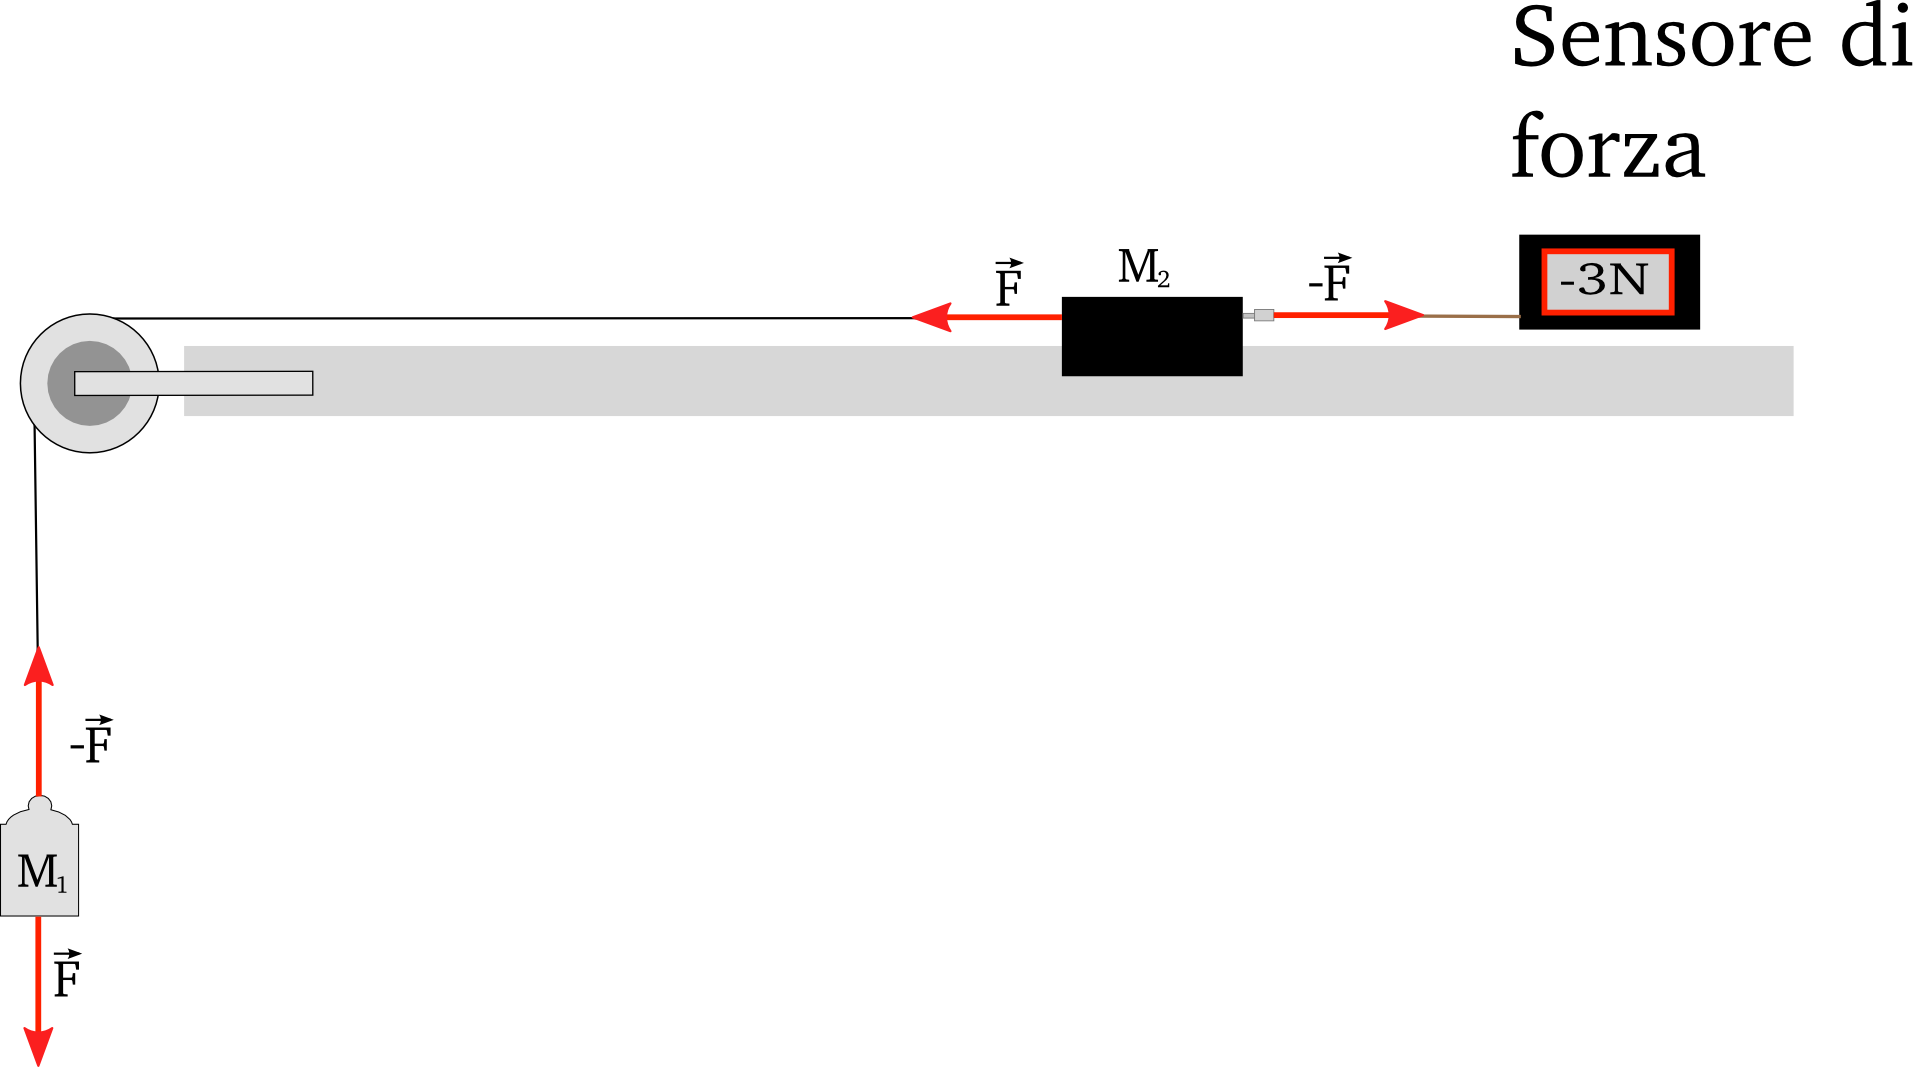
\includegraphics[width=\textwidth]{./Immagini/masse_filo_statico.png}
 % masse_filo_statico.png: 1914x1067 pixel, 200dpi, 24.31x13.55 cm, bb=0 0 689 384
 \caption{Due masse sono collegate tra loro da una fune, il sistema è statico}
 \label{fig:filo_statico}
\end{figure}

\subsection*{Caso dinamico}

Nel caso dinamico il carrello ed il carico sospeso si stanno muovendo con una certa accelerazione $\mathbf{a}$. Come possiamo calcolare il modulo di $\mathbf{a}$?
Per prima cosa notiamo che la forza responsabile del moto delle due masse è unicamente la forza di gravità applicata alla massa sospesa:
\begin{equation}
 \mathbf{F}_g=M_1\mathbf{g}
\end{equation}
questa forza non è applicata unicamente alla massa che sta cadendo, tramite il filo inestensibile è applicata anche alla massa che sta scivolando (quasi) senza attrito sul cuscino d'aria generato dalla guidovia. La seconda legge di Newton ci dice quindi:
\begin{equation}\label{eq:filo_dinamico}
 \mathbf{F}=M_1\mathbf{g}=(M_1+M_2)\mathbf{a}
\end{equation}

l'equazione [\ref{eq:filo_dinamico}] ci permette quindi di ricavare il valore del modulo dell'accelerazione:
\begin{equation}\label{eq:filo_dinamico_res}
 |\mathbf{a}|=\frac{M_1}{M_1+M_2}g
\end{equation}
il risultato [\ref{eq:filo_dinamico_res}] è in accordo con i dati che possiamo raccogliere in laboratorio ed anche con il senso comune, l'accelerazione della massa legata è infatti più piccola di quella che questa avrebbe nel caso cadesse senza alcun collegamento con la massa posta sulla guidovia. Notiamo che a causa della inestensibilità del filo la velocità e l'accelerazione della massa in caduta e di quella in fase di scorrimento devono essere uguali.

\begin{figure}[H]
 \centering
 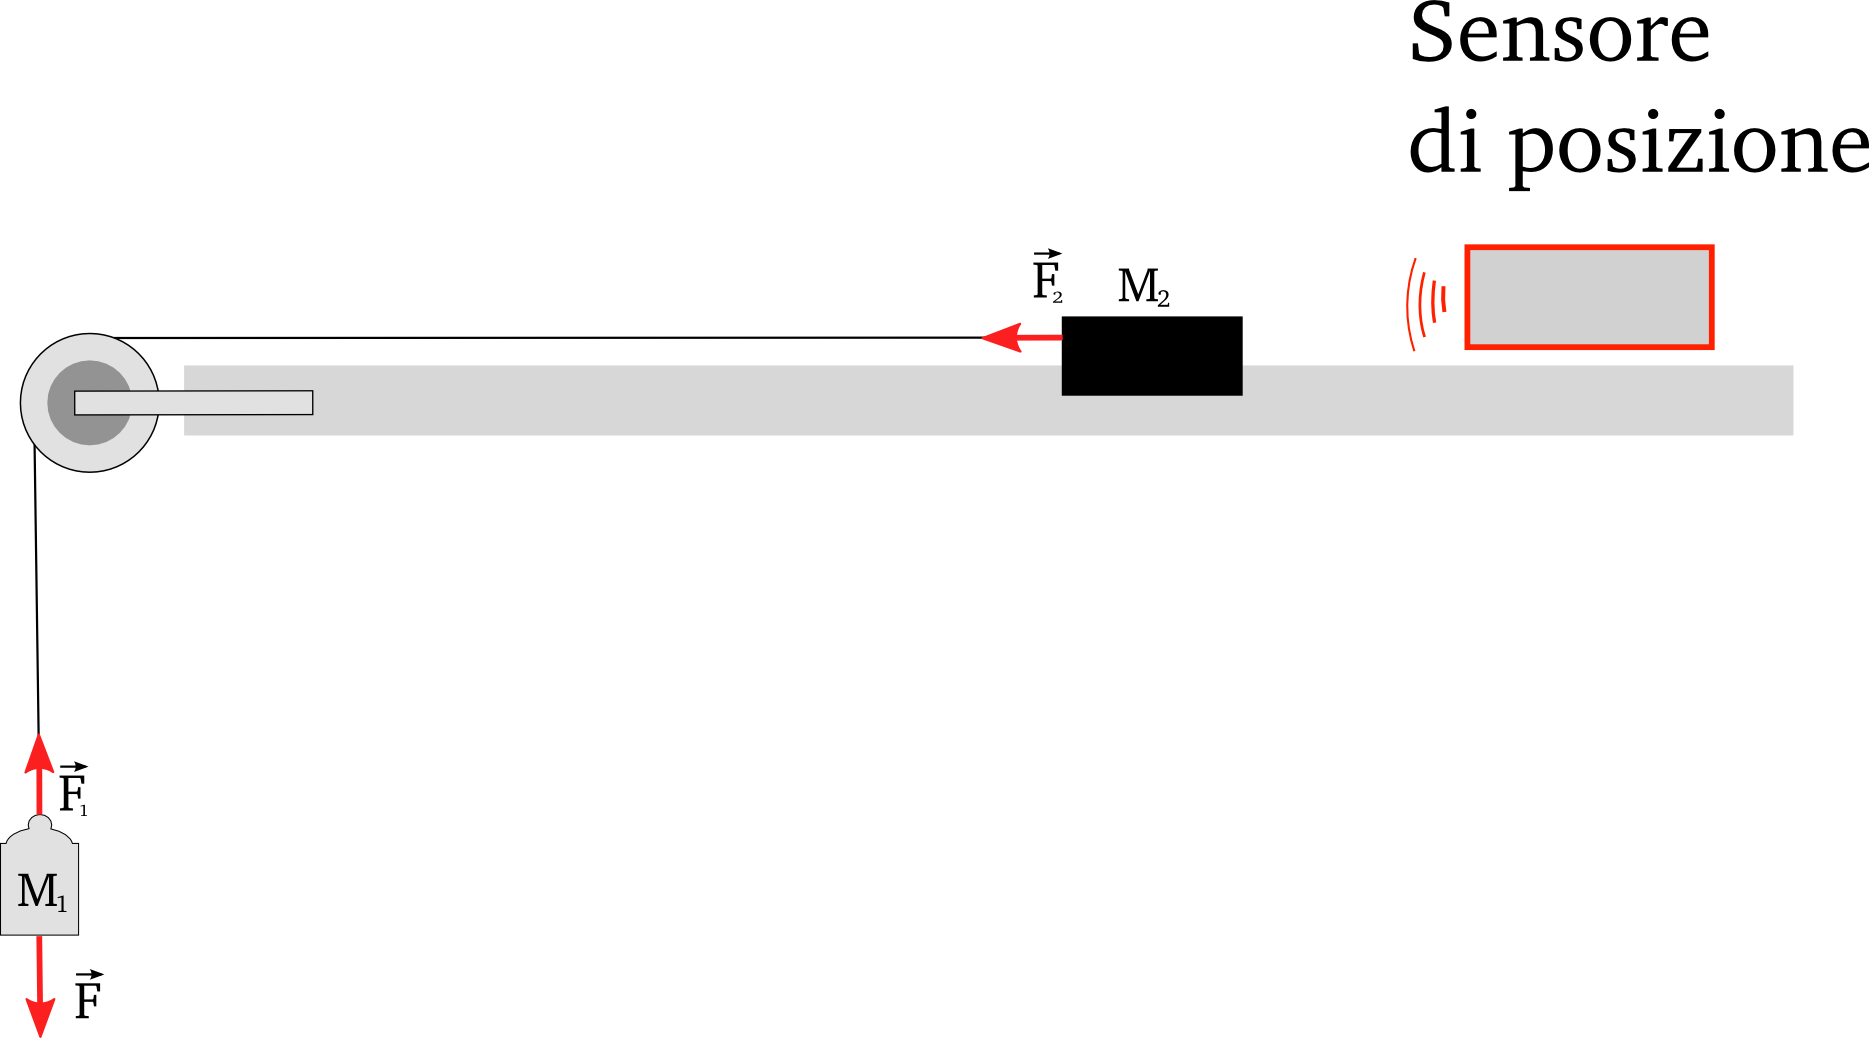
\includegraphics[width=\textwidth]{./Immagini/masse_filo_dinamico.png}
 % masse_filo_dinamico.png: 1869x1038 pixel, 200dpi, 23.74x13.19 cm, bb=
 \caption{Due masse sono collegate da una corda inestensibile e si stanno muovendo verso il basso sotto l'effetto della forza di gravità}
 \label{fig:filo_dinamico}
\end{figure}



\section*{L'attrito radente}

L'esperienza quotidiana sembra contraddire la prima legge di Newton, se infatti lanciamo un oggetto sul tavolo questo dopo un breve lasso di tempo si ferma e non continua il suo moto con velocità costante, come invece ci suggerisce la legge di inerzia.
Per spiegare questo fenomeno dobbiamo supporre che tra l'oggetto e il tavolo ci sia una forza (nota come forza d'attrito) che produce la decelerazione osservata. Si è scoperto sperimentalmente che il modulo di tale forza è:
\begin{equation}
 F_a=\mu F_n
\end{equation}
dove $F_n$ è il modulo della forza normale alla direzione dello spostamento e $\mu$ è il coefficiente d'attrito. È possibile misurare un coefficiente d'attrito statico $\mu_s$ quando il corpo è fermo ed un coefficiente d'attrito dinamico $\mu_d$ quando il corpo è in moto. 
In laboratorio utilizzeremo il sensore di forza per determinare il coefficiente di attrito statico per varie superfici e cercheremo di provare come questo sia indipendente da $F_n$. Nelle misure dovremo quindi per ogni coppia di superfici utilizzate creare una tabella in cui riporteremo la forza premente e la forza d'attrito statico misurata, alla fine dell'esperienza i dati dovranno essere riportati  in un grafico $F_a$ vs $F_n$.

\section*{Misura di g}


Per la misura di $g$ utilizzeremo due sensori a infrarossi come in figura [\ref{fig:gravita_1}]
\begin{figure}[H]
 \centering
 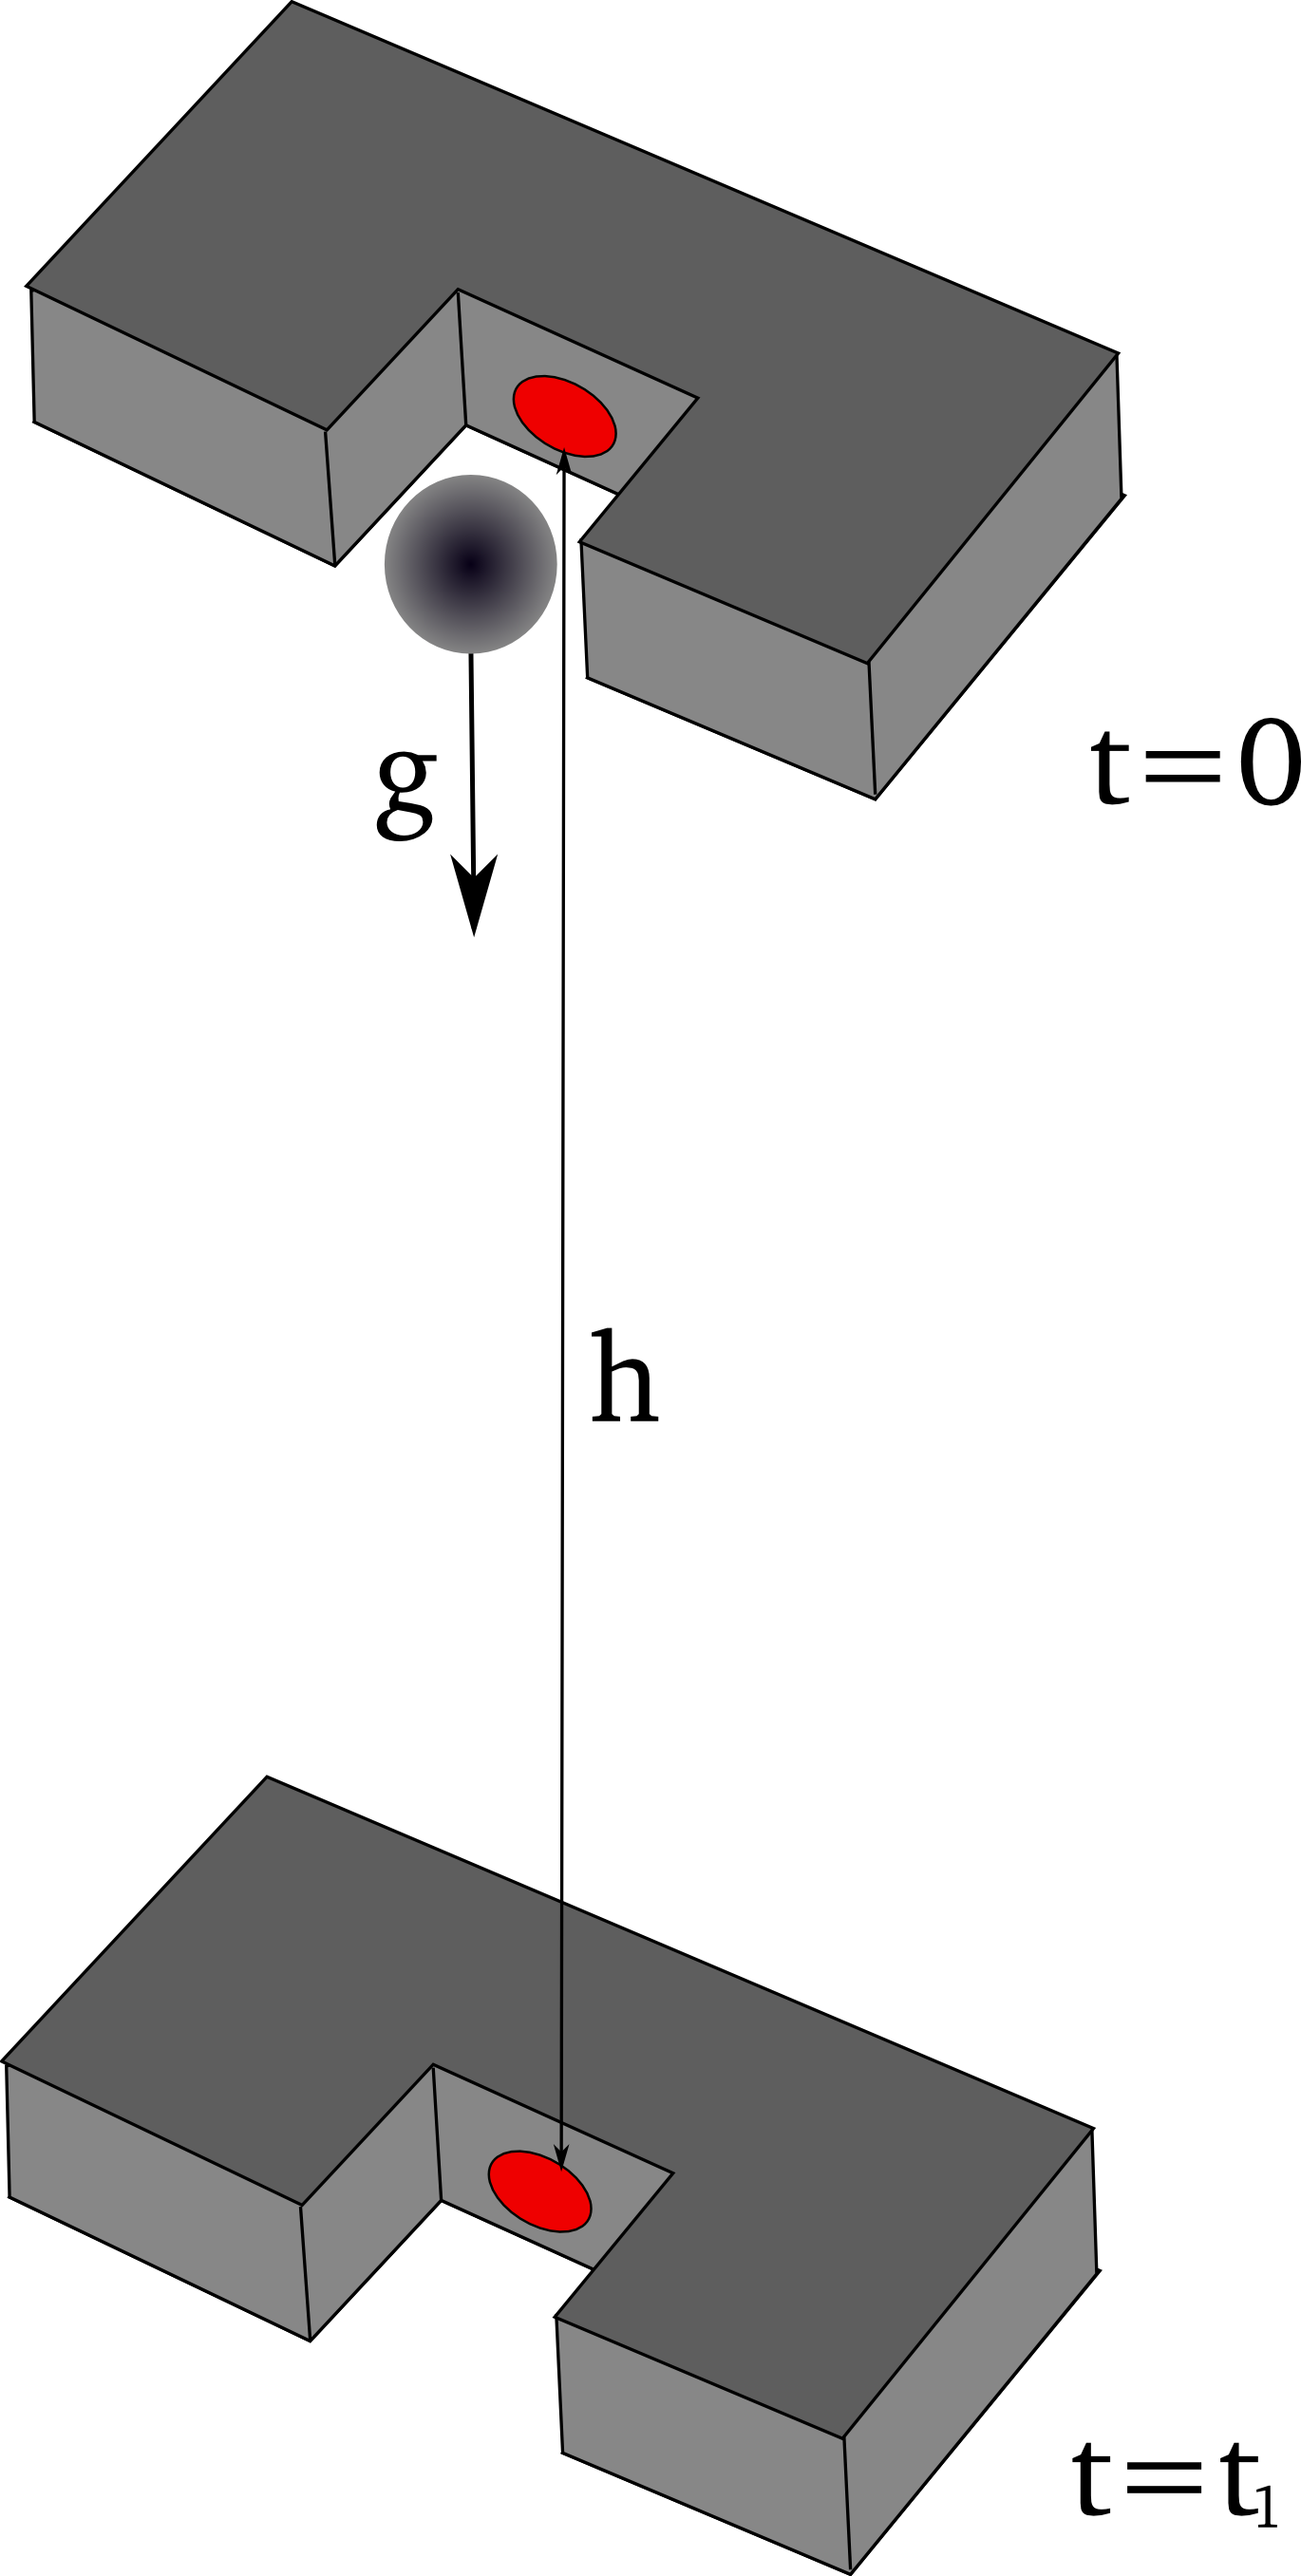
\includegraphics[width=0.3\textwidth]{./Immagini/gravita.png}
 % gravita.png: 1370x2713 pixel, 300dpi, 11.60x22.97 cm, bb=
 \caption{Sensori ad infrarossi per la determinazione del tempo di caduta.}
 \label{fig:gravita_1}
\end{figure}
il cronometro collegato ai rilevatori ad infrarossi ci darà il tempo di caduta, applicando la nota relazione cinematica per il moto uniformemente accelerato:
\begin{equation}
 g=\frac{2s}{t^2}
\end{equation}
possiamo ottenere una stima dell'accelerazione di gravità.
Se il punto di sgancio della massa non coincide con il primo sensore ovvero la massa è stata sganciata da una quota $s_0$ superiore, come da figura [\ref{fig:gravita_2}], il calcolo dell'accelerazione di gravità diventa leggermente più complesso. Dobbiamo prima calcolare la velocità con la quale l'oggetto giunge al termine della prima fotocellula, se la distanza dal punto di sgancio al punto in cui il cronometro inizia a contare il tempo vale $s_0$, la cinematica ci dice che la velocità sarà:
\begin{equation}\label{g_semplice}
 v_0=\sqrt{2gs_0}
\end{equation}

scrivendo l'equazione del moto uniformemente accelerato per il tratto di caduta $s$ compiuto nel tempo $t$, misurato dal cronometro:
\begin{equation}
s=v_0t+\frac 1 2 gt^2=t\sqrt{2gs_0}+\frac{1}{2}gt^2
\end{equation}
da cui otteniamo per l'accelerazione di gravità il valore:
\begin{equation}\label{g_completo}
g=\frac{2(s+2s_0-2\sqrt{ss_0+s_0^2})}{t^2}
\end{equation}


\begin{figure}[H]
 \centering
 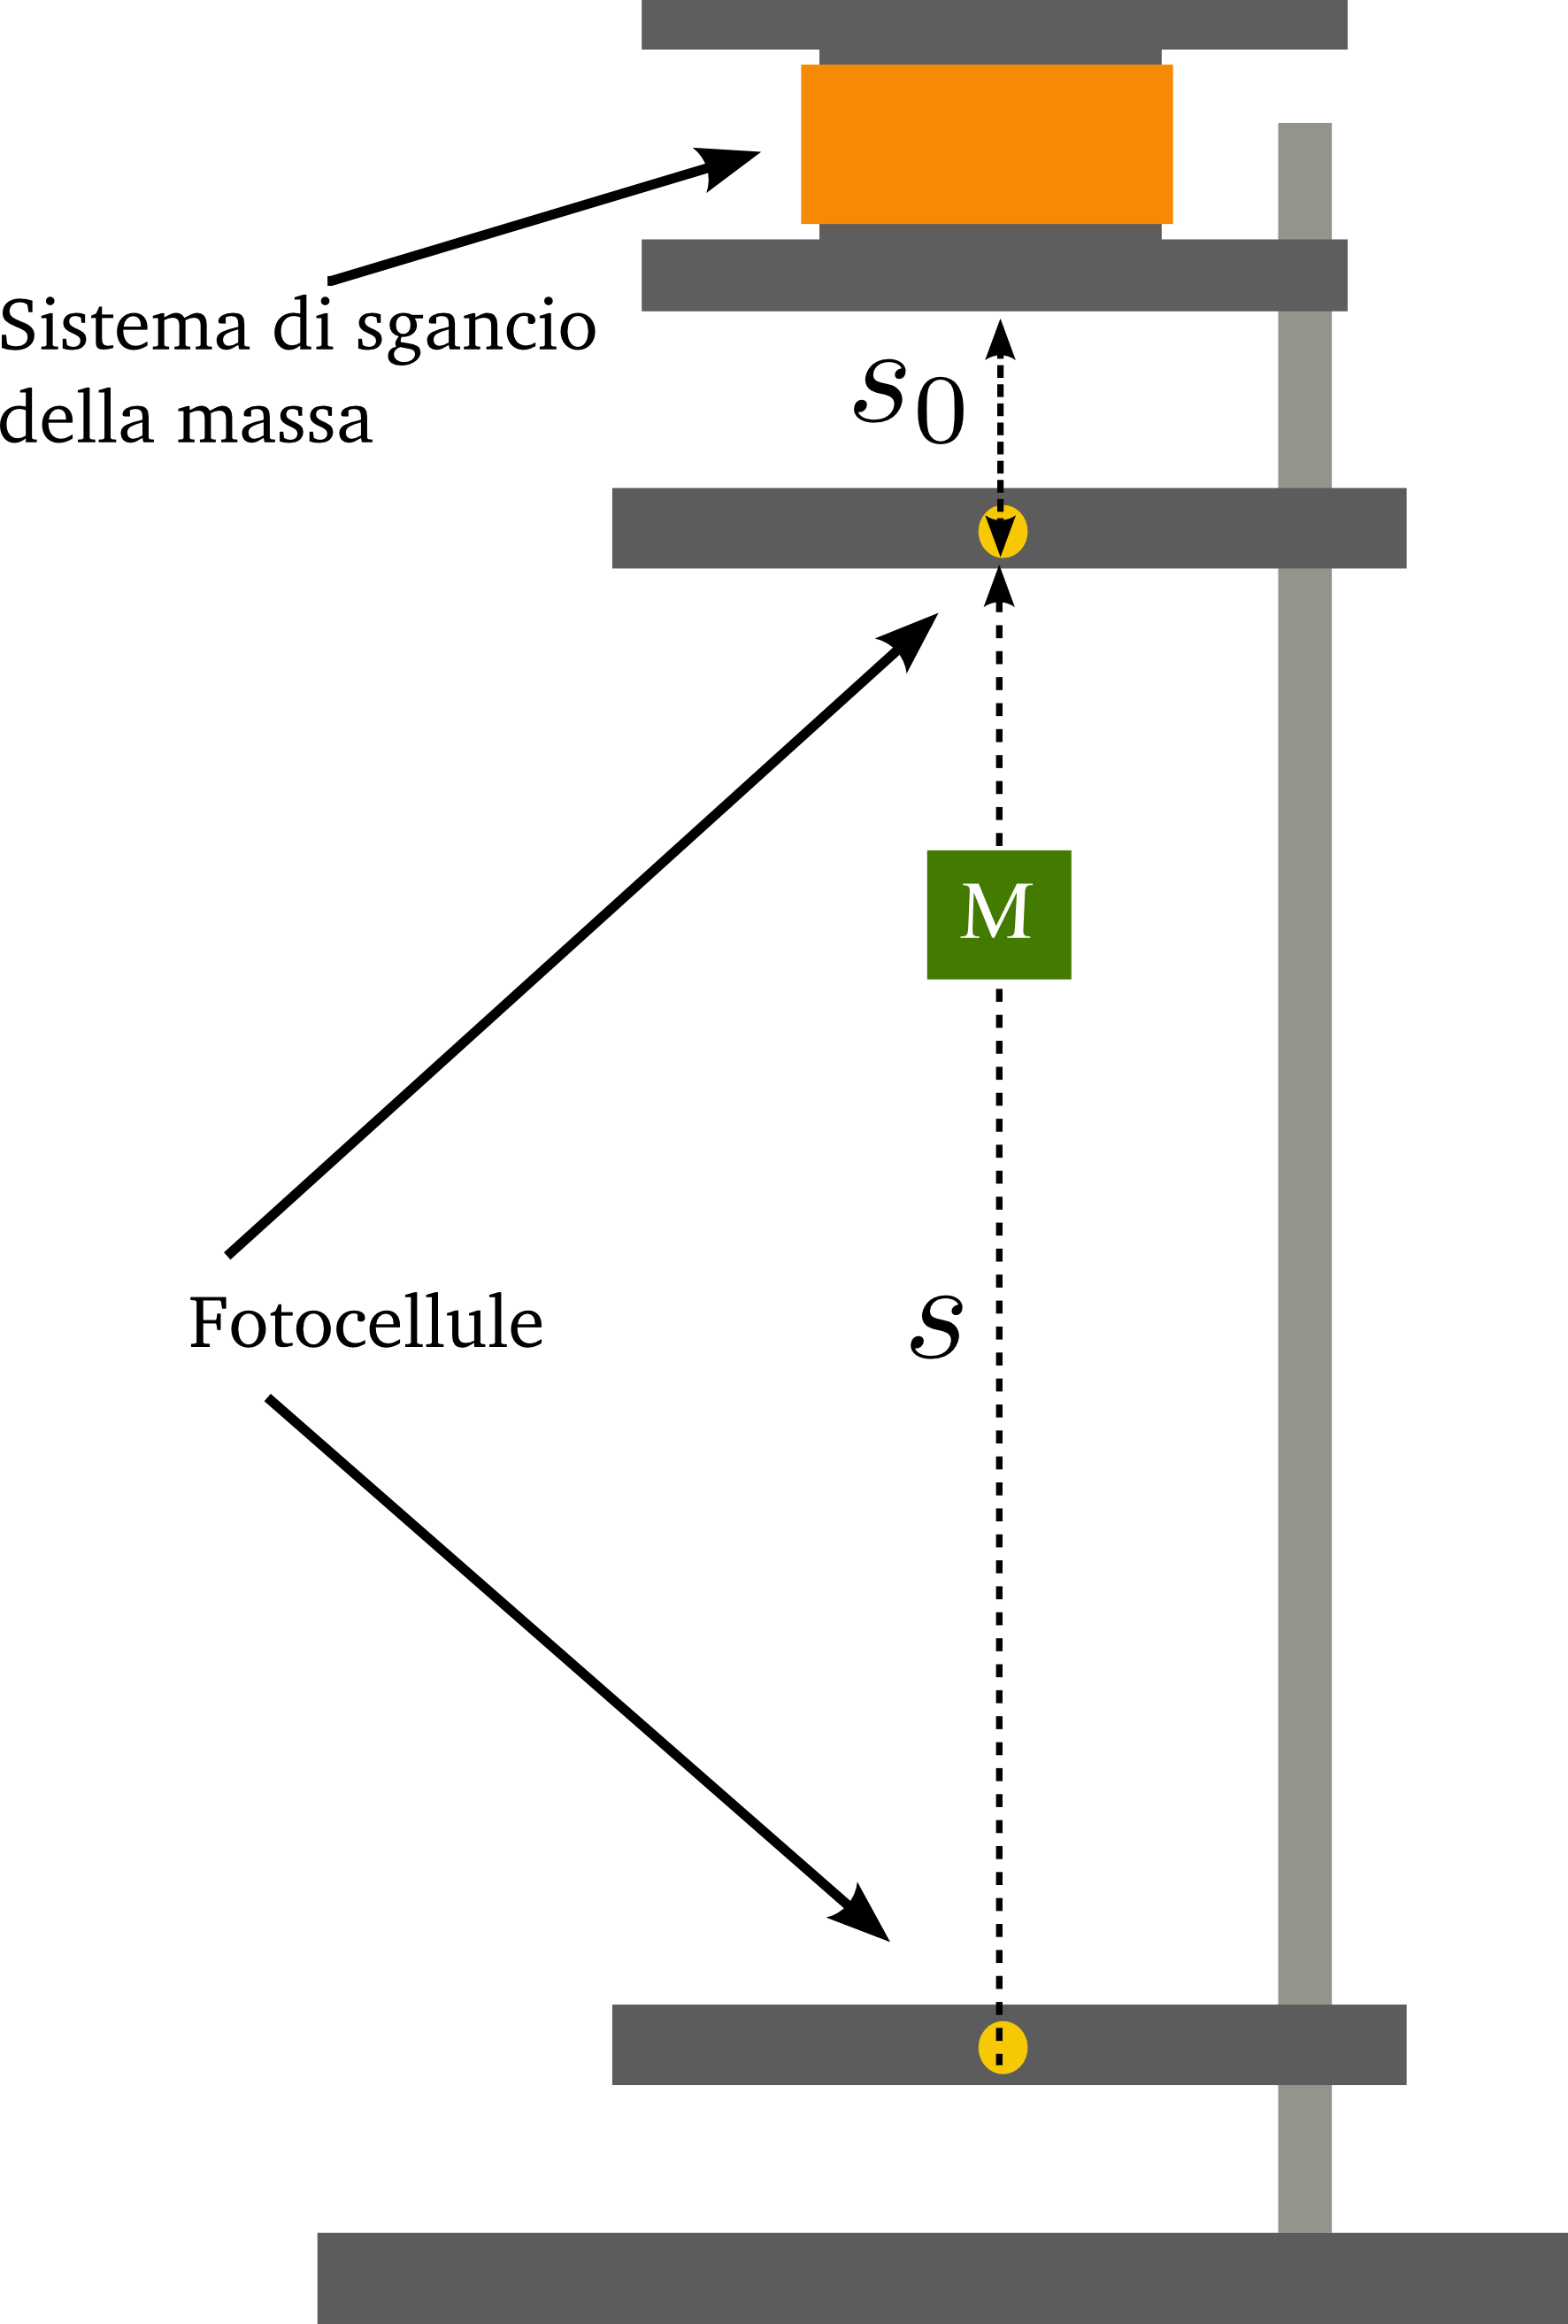
\includegraphics[width=0.5\textwidth]{./Immagini/gravita_2.png}
 % gravita_2.png: 1772x2626 pixel, 270dpi, 16.66x24.69 cm, bb=0 0 472 700
 \caption{Se il punto di sgancio non coincide con la prima fotocellula dobbiamo tenere conto anche del tratto $s_0$ nella determinazione dell'accelerazione di gravità}
 \label{fig:gravita_2}
\end{figure}

vediamo che la [\ref{g_completo}] si riduce alla [\ref{g_semplice}] per $s_0\to 0$


\section*{Il pendolo elastico}

Il pendolo elastico è costituito da una massa $m$ oscillante sotto l'azione della forza di gravità e  della forza elastica $F=-kx$. Sfortunatamente non disponiamo degli strumenti matematici necessari a ricavare la legge oraria e la dipendenza temporale della velocità, è però possibile giungere ad una soluzione soddisfacente del problema, confrontando il moto della massa soggetta alla forza elastica con quello di un oggetto che si muove di moto circolare uniforme.

\begin{figure}[H]
 \centering
 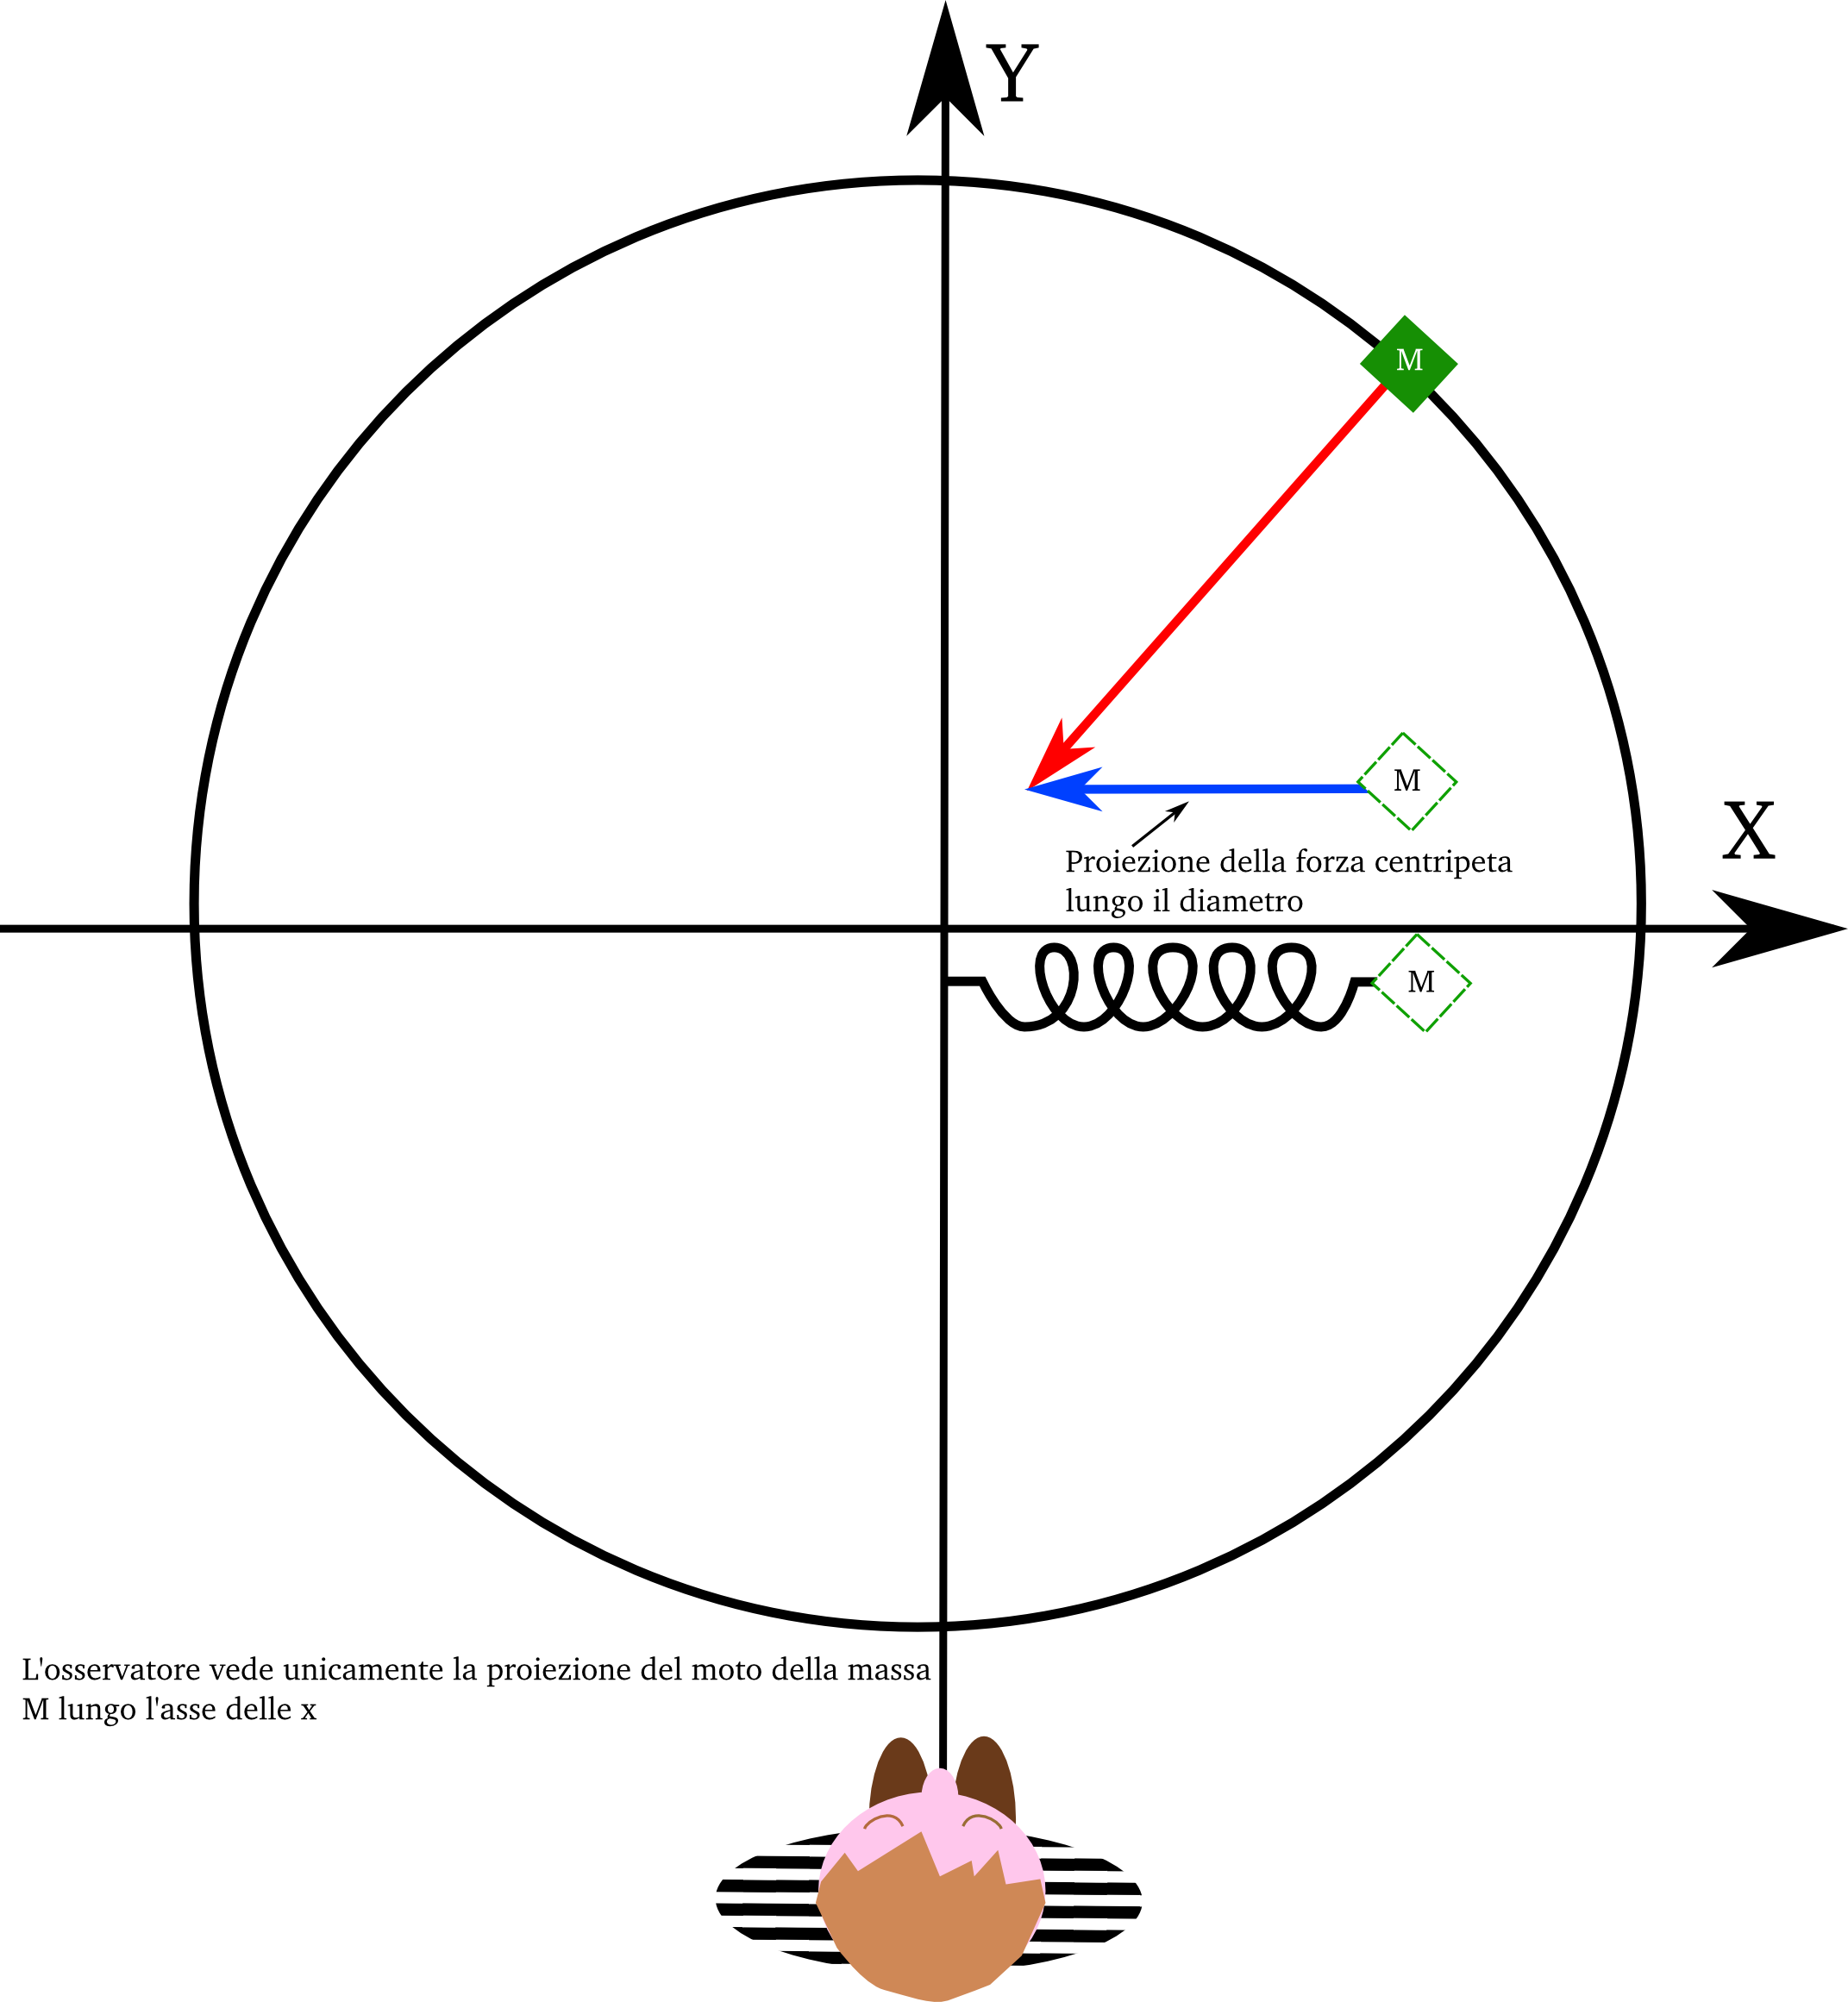
\includegraphics[width=0.8\textwidth]{./Immagini/armonico_vista.png}
 % armonico_vista.png: 1944x2142 pixel, 300dpi, 16.46x18.14 cm, bb=0 0 467 514
 \caption{Un osservatore in grado di osservare unicamente la proiezione del moto lungo l'asse delle ascisse non è in grado di distinguere tra il moto di una massa collegata ad una molla, e quello di un oggetto vincolato ad una circonferenza in rotazione uniforme}\label{fig:armonico1}
\end{figure}


Immaginiamo una massa $m$ in moto con velocità angolare costante lungo una circonferenza di raggio $r$ dalla teoria che abbiamo studiato risulta che la componente $x$ della sua accelerazione centripeta è:
\begin{equation}
 a_x=-\omega^2r\cos(\omega t)
\end{equation}
quindi un osservatore disposto in modo da vedere di taglio la rotazione della massa misurerà una forza:
\begin{equation}
 F_x=-m\omega^2r\cos(\omega t)
\end{equation}

ricordando ora che la componente orizzontale del vettore posizione risulta $ x=r\cos\omega t$ possiamo riscrivere la componente $x$ della forza centripeta come:
\begin{equation}
 F_x=-m\omega^2x
\end{equation}
che, dal punto di vista matematico, ha la stessa forma della legge elastica ovvero una costante che moltiplica uno spostamento $x$:
\begin{equation}
 F_e=-kx
\end{equation}
in particolare se scegliamo $\omega$ in modo che sia:
\begin{equation}
 m\omega^2=k
\end{equation}
ovvero:
\begin{equation}\label{omega1}
 \omega=\sqrt{\frac k m}
\end{equation}
la forza elastica e la componente $x$ della forza centripeta risulteranno numericamente identiche, questo ci assicura che i moti risultanti, della massa collegata alla molla e della massa vincolata alla circonferenza rotante sono identici.
Tale importante osservazione ci permette di ricavare la dipendenza temporale dello spostamento della massa vincolata alla molla e la sua velocità, semplicemente riutilizzando le formule ricavate per il moto circolare.
Analizziamo il caso semplice in cui al tempo $t=0$ la massa collegata alla molla si trova alla massima estensione positiva $\overline x$ ovvero $x(0)=\overline x$. Usando la [\ref{omega1}] e la componente $x$ del vettore posizione del moto circolare uniforme, considerando il raggio della circonferenza associata  pari a $\overline x$, possiamo scrivere:
\begin{equation}
 x=\overline x \cos(\omega t)
\end{equation}
e quindi
\begin{equation}
 x=\overline x\cos(\sqrt{\frac k m}t)
\end{equation}
lo stesso discorso si può fare per la velocità, la componente $x$ della velocità della massa collegata alla circonferenza risulta:
\begin{equation}
 v_x=-\omega \overline x\sin(\omega t)
\end{equation}
per cui la velocità della massa collegata alla molla sarà:
\begin{equation}
 v=-\sqrt{\frac k m }\overline x\sin(\sqrt{\frac k m }t)
\end{equation}

\subsection*{Diverse condizioni iniziali}
Nell'esempio precedente abbiamo supposto che la massa fosse lasciata libera al tempo zero con velocità iniziale nulla; se invece decidessimo di impartirle una velocità iniziale diversa da zero cosa succederebbe? Cerchiamo di analizzare il problema utilizzando un esempio. Trattiamo il caso della massa lasciata partire dalla posizione $x=0$ al tempo $t=0$ con velocità iniziale $v_0$.
L'allungamento massimo della molla risulta pari a:
\begin{equation}
 \overline x=\frac{v_0}{\omega}
\end{equation}
Quali saranno le equazioni che descrivono il moto della massa? Notiamo che all'istante $t=0$ la massa deve trovarsi nell'origine quindi l'equazione $x=\overline x\cos(\omega t)$ non sarà più adatta a descrivere il moto\footnote{Infatti il coseno non è mai nullo per argomento nullo} , come possiamo risolvere il problema? Una strada per giungere alla soluzione, senza utilizzare della matematica complessa, è di pensare che il moto in esame non sia altro che un moto iniziato con massa ferma ad una certa distanza dal punto $x=0$ in un tempo \textbf{anteriore} rispetto a quando facciamo partire il cronometro. Immaginate, ad esempio, che qualcuno abbia fatto partire la massa senza dirvi nulla, che la luce del laboratorio sia spenta e che questa venga accesa all'istante del vostro orologio $t=0$  quando la massa si trova a passare per $x=0$ con una certa velocità $v_0$, potremmo quindi pensare che il nostro esperimento con condizioni iniziali diverse non sia altro che il moto semplice già studiato ma iniziato in un tempo $t_0$ anteriore rispetto a quello in cui abbiamo fatto partire il nostro cronometro.
Scriveremo quindi per la posizione $x$ della massa al tempo $t$ la relazione:
\begin{equation}\label{mot_trasl}
 x=\overline x\cos(\omega(t-t_0))
\end{equation}
Quando deve essere iniziato il movimento della massa affinché al tempo $t=0$ questa si trovi nella posizione $x=0$? Per rispondere a questa domanda dobbiamo determinare quando la funzione coseno si annulla. Da quanto avete studiato in matematica sapete che il coseno si annulla in $\frac \pi 2 +k\pi$ quindi per trovare il tempo $t_0$ minimo devo semplicemente uguagliare a $\frac \pi 2 $ l'argomento del coseno nella [\ref{mot_trasl}], ponendo $t=0$:
\begin{equation}
 -\omega t_0=\frac \pi 2
\end{equation}
da cui
\begin{equation}\label{t0}
 t_0=-\frac{\pi}{2\omega}
\end{equation}
Se ricordiamo quanto detto precedentemente, ovvero che $\omega$ rappresenta la pulsazione del moto armonico semplice e che il periodo è pari a:
\begin{equation}
 T=\frac{2\pi}{\omega}
\end{equation}
otteniamo:
\begin{equation}
 t_0=-\frac{T}{4}
\end{equation}
ovvero il moto deve essere iniziato un quarto di periodo prima dell'inizio della misura. Armati di queste informazioni possiamo riscrivere la [\ref{mot_trasl}] sostituendo al posto del tempo iniziale il valore trovato nella [\ref{t0}]:
\begin{equation}
 x=\overline x \cos(\omega t-\omega \frac{\pi}{2\omega})=\overline x \cos(\omega t-\frac \pi 2)
\end{equation}
che ricordando gli archi associati si riduce a :
\begin{equation}
 x=\overline x\sin\omega t
\end{equation}
Durante l'esperienza di laboratorio vedremo cosa succederà in casi diversi quando al tempo $t=0$ la posizione della massa non è nulla ne lo è la sua velocità.

\subsection*{Caso reale molla dotata di massa}
Analizziamo ora l'oscillatore verticale e vediamo che può essere descritto utilizzando la tecnica studiata nei paragrafi precedenti. Quando appendiamo la massa $M$ alla molla questa si allungherà di una certa quantità e raggiungerà la coordinata $\overline x$, l'allungamento della molla (vedi figura [\ref{fig:armonico1}]) sarà\footnote{Notate che abbiamo utilizzato la coordinata $\overline x_0$ come punto di non estensione della molla nei calcoli effettuati, cioè si è supposto che tutti i moti avvengano rispetto alla coordinata $x$ della molla allungata sotto il suo stesso peso}:
\begin{equation}
 \xi_{eq}=\overline x-\overline x_0
\end{equation}
per cui all'equilibrio varrà la relazione:
\begin{equation}\label{equiv_molla_1}
 mg-k\xi_{eq}=0
\end{equation}
cioè la forza elastica della molla controbilancia la forza di gravità. Per un generico allungamento della mola $\xi=x-\overline x_0$ la forza che agisce sulla massa sospesa $M$ sarà:
\begin{equation}\label{equiv_molla_2}
 F=mg-k\xi
\end{equation}
se ora sostituiamo nella [\ref{equiv_molla_2}] la [\ref{equiv_molla_1}] otteniamo:
\begin{equation}
 F=k\xi_{eq}-k\xi=k\overline x -k\overline x_0-kx+k\overline x_0=k\overline x-kx=-k(x-\overline x)
\end{equation}
sostituendo poi a $x-\overline x$ la nuova variabile $z$ possiamo scrivere:
\begin{equation}
 F=-kz
\end{equation}
ovvero il moto di una molla ideale in cui lo zero della coordinata è la quota di equilibrio della massa sospesa.
In un sistema oscillante massa-molla reale non possiamo prescindere dal considerare la massa della molla che sorregge il carico.
Si può dimostrare che l'allungamento di una molla reale di massa $m$, costante elastica $k$ a cui viene appesa una massa  $M$ è:
\begin{equation}\label{spost_reale}
 \Delta l=g\frac{M+m/2}{k}
\end{equation}
ovvero possiamo immaginare di aver sospeso ad una molla ideale una massa \emph{equivalente} pari a $M+
m/2$.
Durante l'esperimento l'unico dato noto sarà l'accelerazione di gravità dovremo quindi, prima di procedere all'osservazione delle oscillazioni della massa, misurare la costante elastica della molla che andremo ad utilizzare. Facendo riferimento alla figura [\ref{fig:pendolo_reale}] per la determinazione di $k$ dovranno essere eseguite due misure, utilizzando due masse sospese $M_1$ ed $M_2$. Riscriviamo la [\ref{spost_reale}] nel primo caso:
\begin{equation}
 \Delta l_1=x_0-x_1=g\frac{M_1+m/2}{k}
\end{equation}
e nel secondo caso:
\begin{equation}
 \Delta l_2=x_0-x_2=g\frac{M_2+m/2}{k}
\end{equation}
immaginando che sia $M_2>M_1$ calcoliamo la differenza dei due spostamenti:
\begin{equation}
 \Delta l_2-\Delta l_1=x_0-x_2-x_0+x_1=x_1-x_2=g\frac{M_2-M_1}{k}
\end{equation}
dove $x_1$ è la quota misurata dal sensore di posizione del punto di equilibrio del sistema per la massa $M_1$ mentre $x_2$ rappresenta il punto di equilibrio per la massa $M_2$. Notiamo anche che se il sistema massa molla è appeso ad un sensore di forza la differenza delle forze misurate dal sensore $F_2-F_1$ sarà uguale a $g(M_2-M_1)$\footnote{Per quale motivo questa affermazione è vera?}. La costante elastica può quindi essere calcolata in funzione delle quantità misurate $F_1,\ F_2,\ x_1,\ x_2$ come:
\begin{equation}
 k=\frac{F_2-F_1}{x_1-x_2}
\end{equation}


\begin{figure}[H]
 \centering
 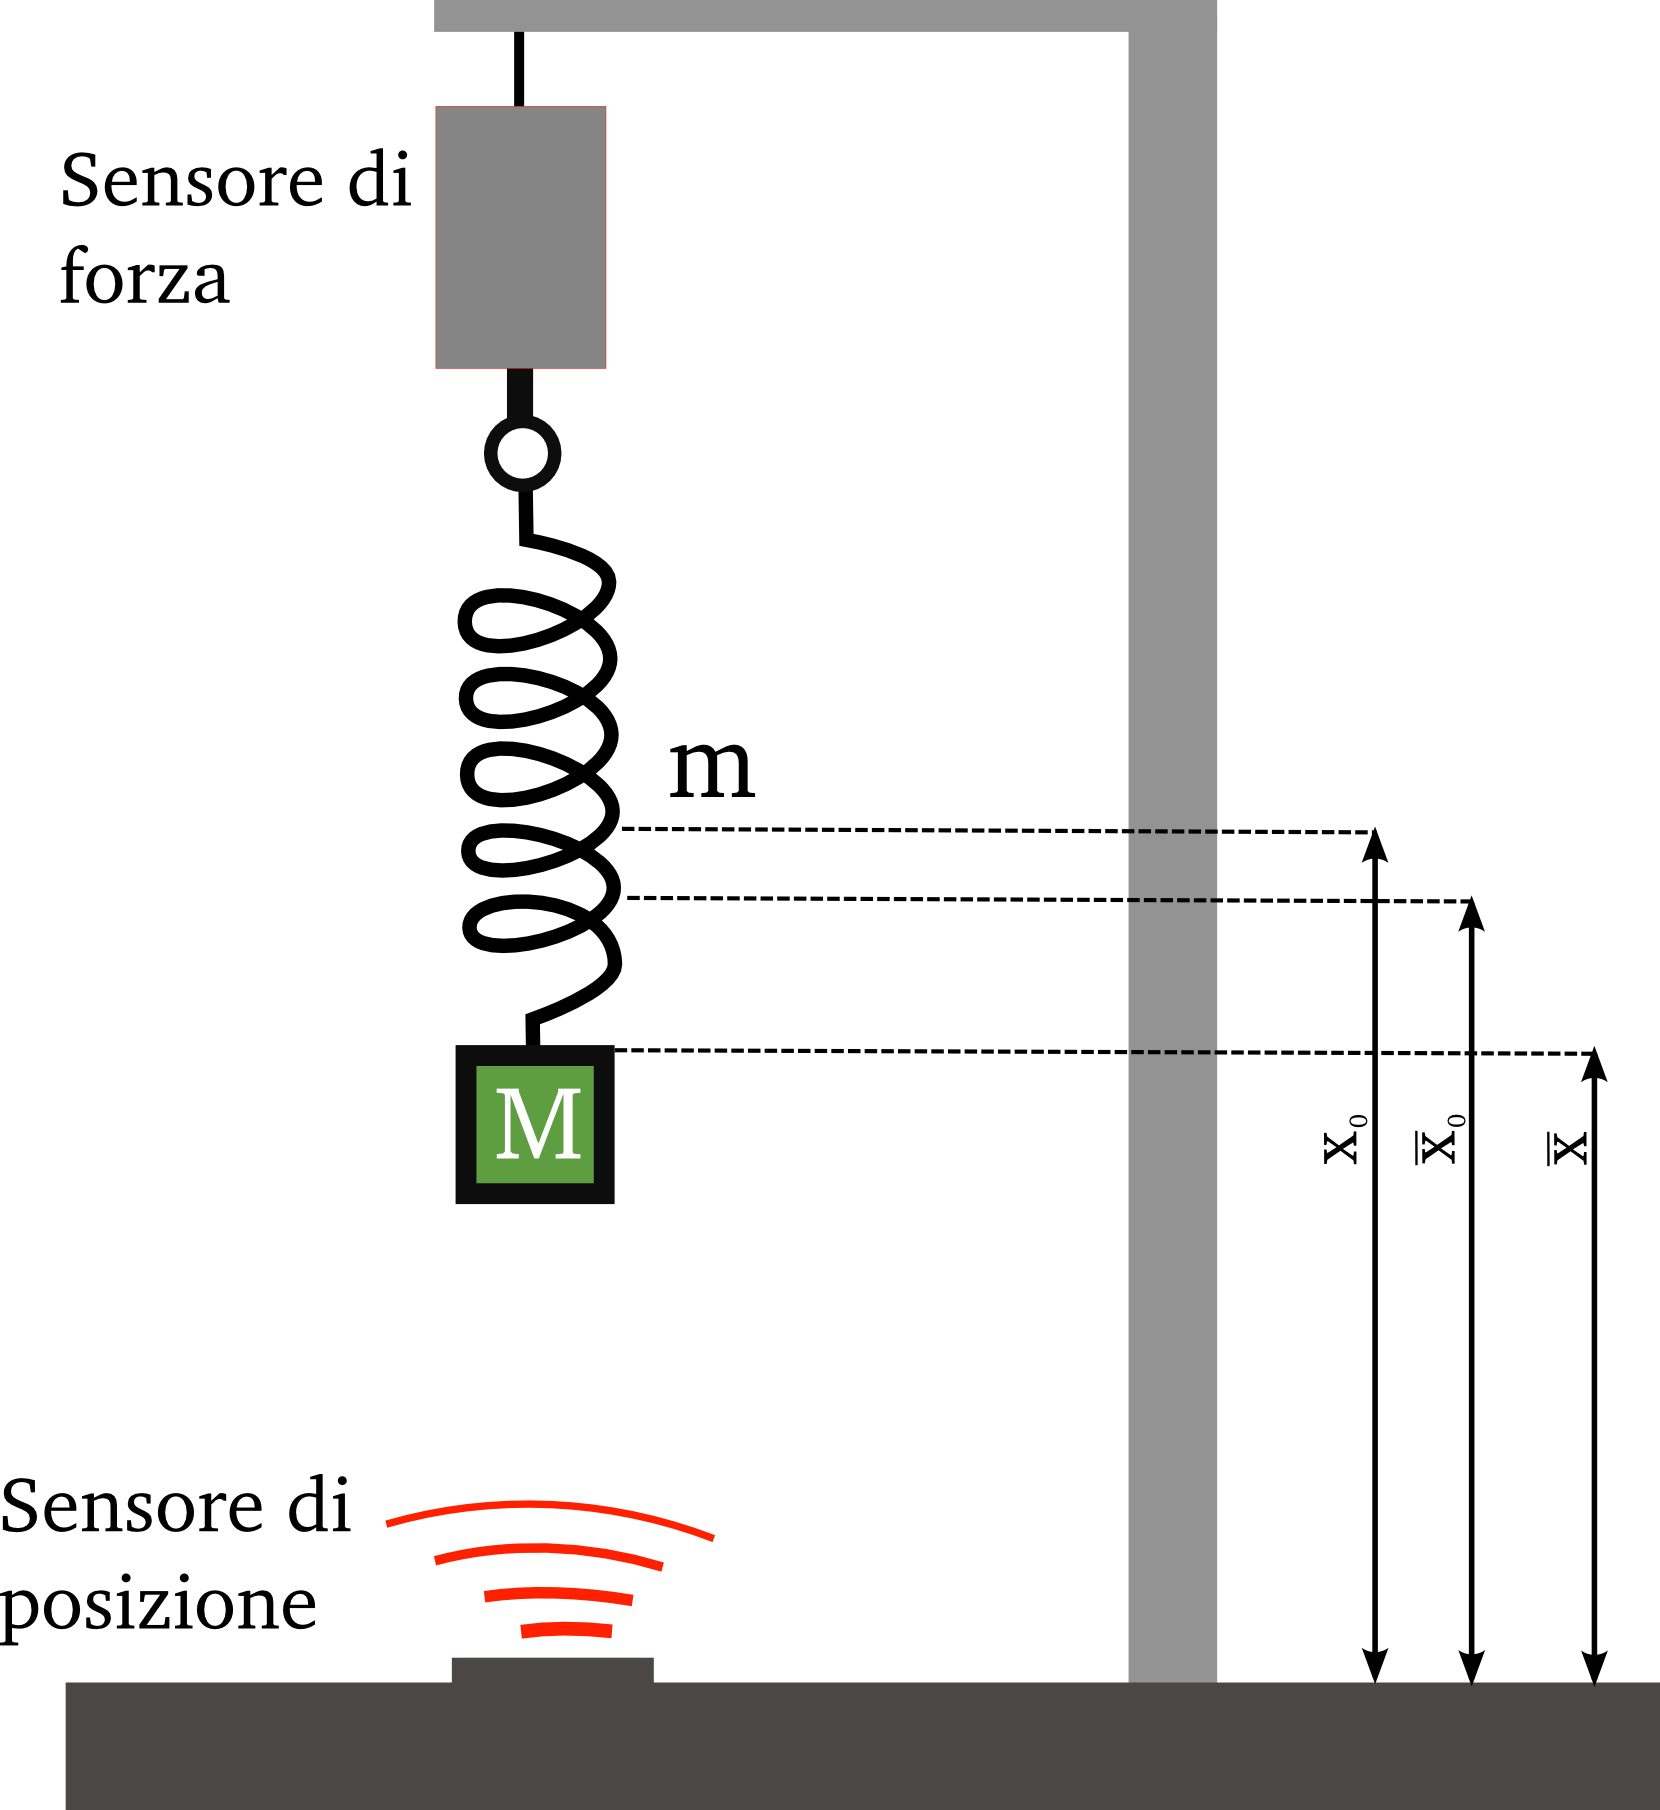
\includegraphics[width=0.7\textwidth]{./Immagini/pendolo_elastica.png}
 % pendolo_elastica.png: 1660x1810 pixel, 72dpi, 58.56x63.85 cm, bb=0 0 1660 1810
\caption{In figura $x_0$ rappresenta la posizione di riposo della molla in assenza di forze, $\overline{x}_0$ la posizione di riposo della molla allungata sotto il suo peso ed $\overline x$ la posizione di equilibrio della molla allungata dalla massa $M$} \label{fig:pendolo_reale}
\end{figure}


Dopo aver determinato la costante elastica della molla dobbiamo iniziare ad osservare il moto oscillatorio del sistema. Per far questo allunghiamo la molla di una quantità arbitraria $\Delta l$ e lasciamola libera di oscillare, campioniamo al computer le posizioni della massa oscillante, per quanto detto precedentemente la variazione della posizione $x$ della massa collegata alla molla presenterà un andamento periodico sinusoidale. La variabile $x$ non assume mai il valore $0$, perché?
Cosa dobbiamo fare per far si che il nostro sistema possa essere descritto da una funzione sinusoidale del tipo $A\cos(\omega(t-t_0))$? Il periodo del sistema dipende dall'ampiezza dell'oscillazione?
Analizzando i dati vi accorgerete che il periodo del sistema oscillante non è uguale a quello del sistema teorico, in cui la molla è priva di massa, che ricordiamo essere
\begin{equation}
 T=2\pi\sqrt{\frac{M}{k}}
\end{equation}
ma per molle sufficientemente rigide vale:
\begin{equation}
 T=2\pi\sqrt{\frac{M+m/3}{k}}
\end{equation}

ovvero il sistema si comporta come un sistema ideale in cui la massa appesa alla molla è aumentata di un terzo della massa della molla stessa. Sarà vostro compito evidenziare questa discrepanza dovuta alla massa finita della molla.


\section*{L'attrito viscoso}

Quando un corpo di dimensioni finite cade all'interno di un gas o di un liquido sente una forza di attrito che si oppone al suo moto e che dipende, secondo varie leggi, dalla velocità. In questo esperimento studieremo la forza di attrito che l'aria oppone al moto di un corpo. Sperimentalmente si può osservare che se un oggetto si muove lentamente\footnote{Per applicare [\ref{visc_1}] il moto del fluido attorno all'oggetto deve essere con buona approssimazione laminare} all'interno di un gas o di un liquido la forza di attrito che si oppone al suo moto
\begin{equation}\label{visc_1}
 F=-\gamma v
\end{equation}
dove $\gamma$ rappresenta il coefficiente di attrito viscoso in regime laminare e $v$ la velocità del corpo.
Se la velocità è sufficientemente elevata la forza di attrito non è più proporzionale ad essa ma al suo quadrato e segue la legge empirica:
\begin{equation}
 F=-\frac{1}{2}C\rho A v^2
\end{equation}
dove $C$ rappresenta il coefficiente aerodinamico di trascinamento, $\rho$\footnote{La densità $\rho$ dell'aria alla temperatura di $20°$ al livello del mare è circa $1.2kgm^{-3}$} la densità del mezzo entro cui il corpo si muove e $A$ la sezione d'urto del corpo in caduta.
In questo esperimento cercheremo di determinare la dipendenza quadratica o lineare della forza di attrito dalla velocità. Per far questo misureremo l'accelerazione cui è sottoposta una massa in caduta libera. Dalla seconda legge di Newton sappiamo che:
\begin{equation}
 F=ma
\end{equation}
nel nostro caso la forza sarà data dalla somma di forza di gravità e di forza di attrito:
\begin{equation}
 F=mg-F_a
\end{equation}
dove $F_a$ rappresenta il modulo della forza di attrito. Dalla misura di $a$ e della massa $M$  possiamo quindi scrivere:
\begin{equation}
F_a=mg-ma
\end{equation}
ovvero nel caso di dipendenza lineare
\begin{equation}
\gamma v=mg-ma
\end{equation}
mentre in quello di dipendenza quadratica
\begin{equation}
 \frac{1}{2}C\rho A v^2=mg-ma
\end{equation}


\subsection*{Misura della posizione verticale}
Per misurare la posizione verticale di una massa in caduta, utilizzeremo un circuito simile a quello di figura [\ref{fig:misura_verticale}]. Il sistema è molto semplice ed è costituto da:
\begin{itemize}
 \item Un cilindro di rame forato al cui interno è stato alloggiato un piccolo tubo in plastica
 \item Una resistenza a filo (costantana) tesa tra il soffitto e il pavimento
 \item Un generatore di tensione
 \item Un voltmetro collegato al sistema di acquisizione dati 
\end{itemize}
\begin{figure}[H]
 \centering
 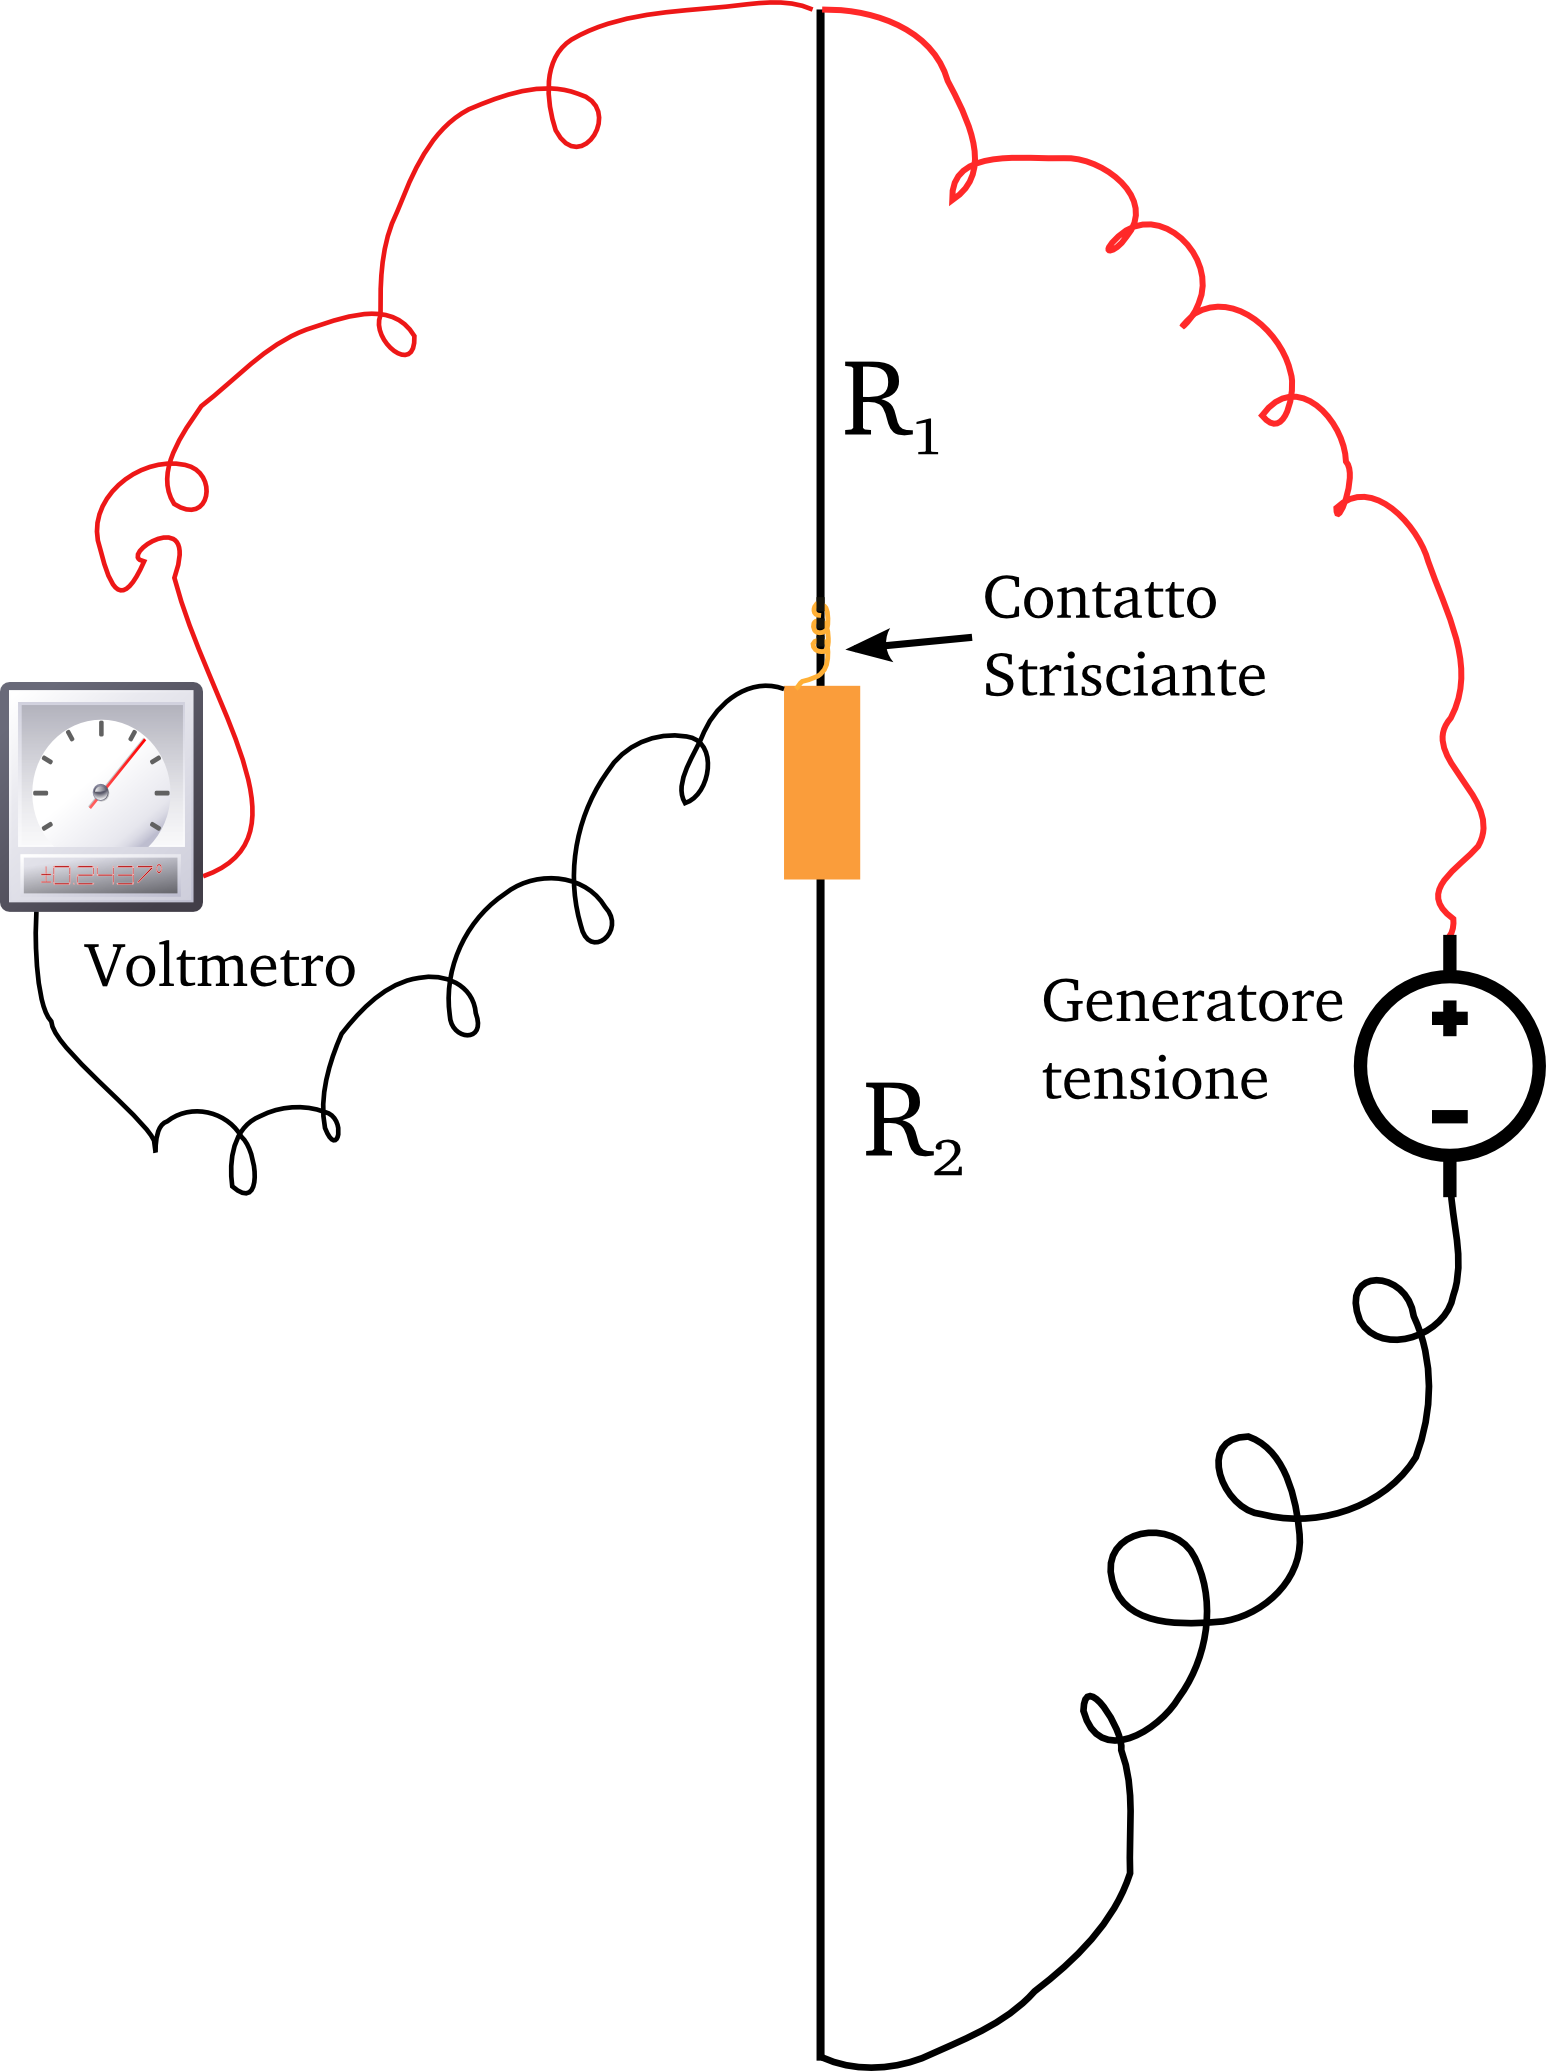
\includegraphics[width=0.6\textwidth]{./Immagini/misura_posizione_verticale.png}
 % misura_posizione_verticale.png: 1553x2071 pixel, 200dpi, 19.72x26.30 cm, bb=0 0 559 746
\caption{Rappresentazione schematica del sistema per la misura dello spostamento verticale} \label{fig:misura_verticale}
\end{figure}
Nello schema elettrico di figura [\ref{fig:schema_elettrico}] la resistenza $R_2$ rappresenta il segmento di filo resistivo che va dal pavimento alla posizione attuale della sonda verticale, per migliorare la qualità delle misure\footnote{Sapreste dire perché?} la resistenza è stata chiusa su un condensatore da $22nF$.
\begin{figure}[H]
 \centering
 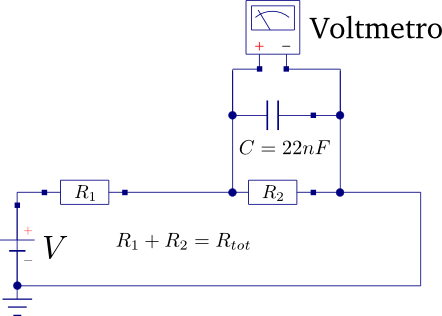
\includegraphics[width=0.7\textwidth]{./Immagini/schema_misura_verticale.png}
 % schema_misura_verticale.png: 452x677 pixel, 250dpi, 4.59x6.88 cm, bb=0 0 130 195
 \caption{Lo schema elettrico del sistema di misura}
 \label{fig:schema_elettrico}
\end{figure}
Questo sistema di misura ci fornisce dei valori in volt, noi siamo però interessati a delle misure di lunghezza, fortunatamente la differenza di potenziale misurata e la lunghezza della resistenza sono proporzionali ovvero vale una legge del tipo:
\begin{equation}\label{ohm}
 V\propto y
\end{equation}
dove $y$ è la lunghezza della resistenza $R_2$. Per calibrare il sensore, al fine di misurare delle lunghezze, posizioniamo la sonda alla massima altezza e tramite il voltmetro misuriamo la differenza di potenziale, otteniamo una coppia $(V_0,y_0)$, ripetiamo poi la procedura per il punto più basso raggiungibile dalla sonda ed otteniamo un'altra coppia $(V_1,y_1)$ in virtù della linearità della relazione [\ref{ohm}] calcoliamo il coefficiente di proporzionalità tra la tensione e la lunghezza della resistenza:
\begin{equation}
 w=\frac{V_0-V_1}{y_0-y_1}
\end{equation}
da cui
\begin{equation}
y=\frac V w 
\end{equation}
una volta determinato il valore della costante $w$ sarà sufficiente inserirlo all'interno del programma di acquisizione dati per visualizzare, in vece della tensione, la quota della sonda.
Come ultima cosa notiamo che lo zero della coordinata $y$ si trova nel punto in cui il polo negativo del generatore di tensione è saldato al filo resistivo, essendo finita la lunghezza della sonda questa coordinata non sarà mai raggiungibile. Notiamo anche che la coordinata $y$ aumenta, secondo la nostra definizione, dal basso verso l'alto.

\begin{figure}[H]
 \centering
 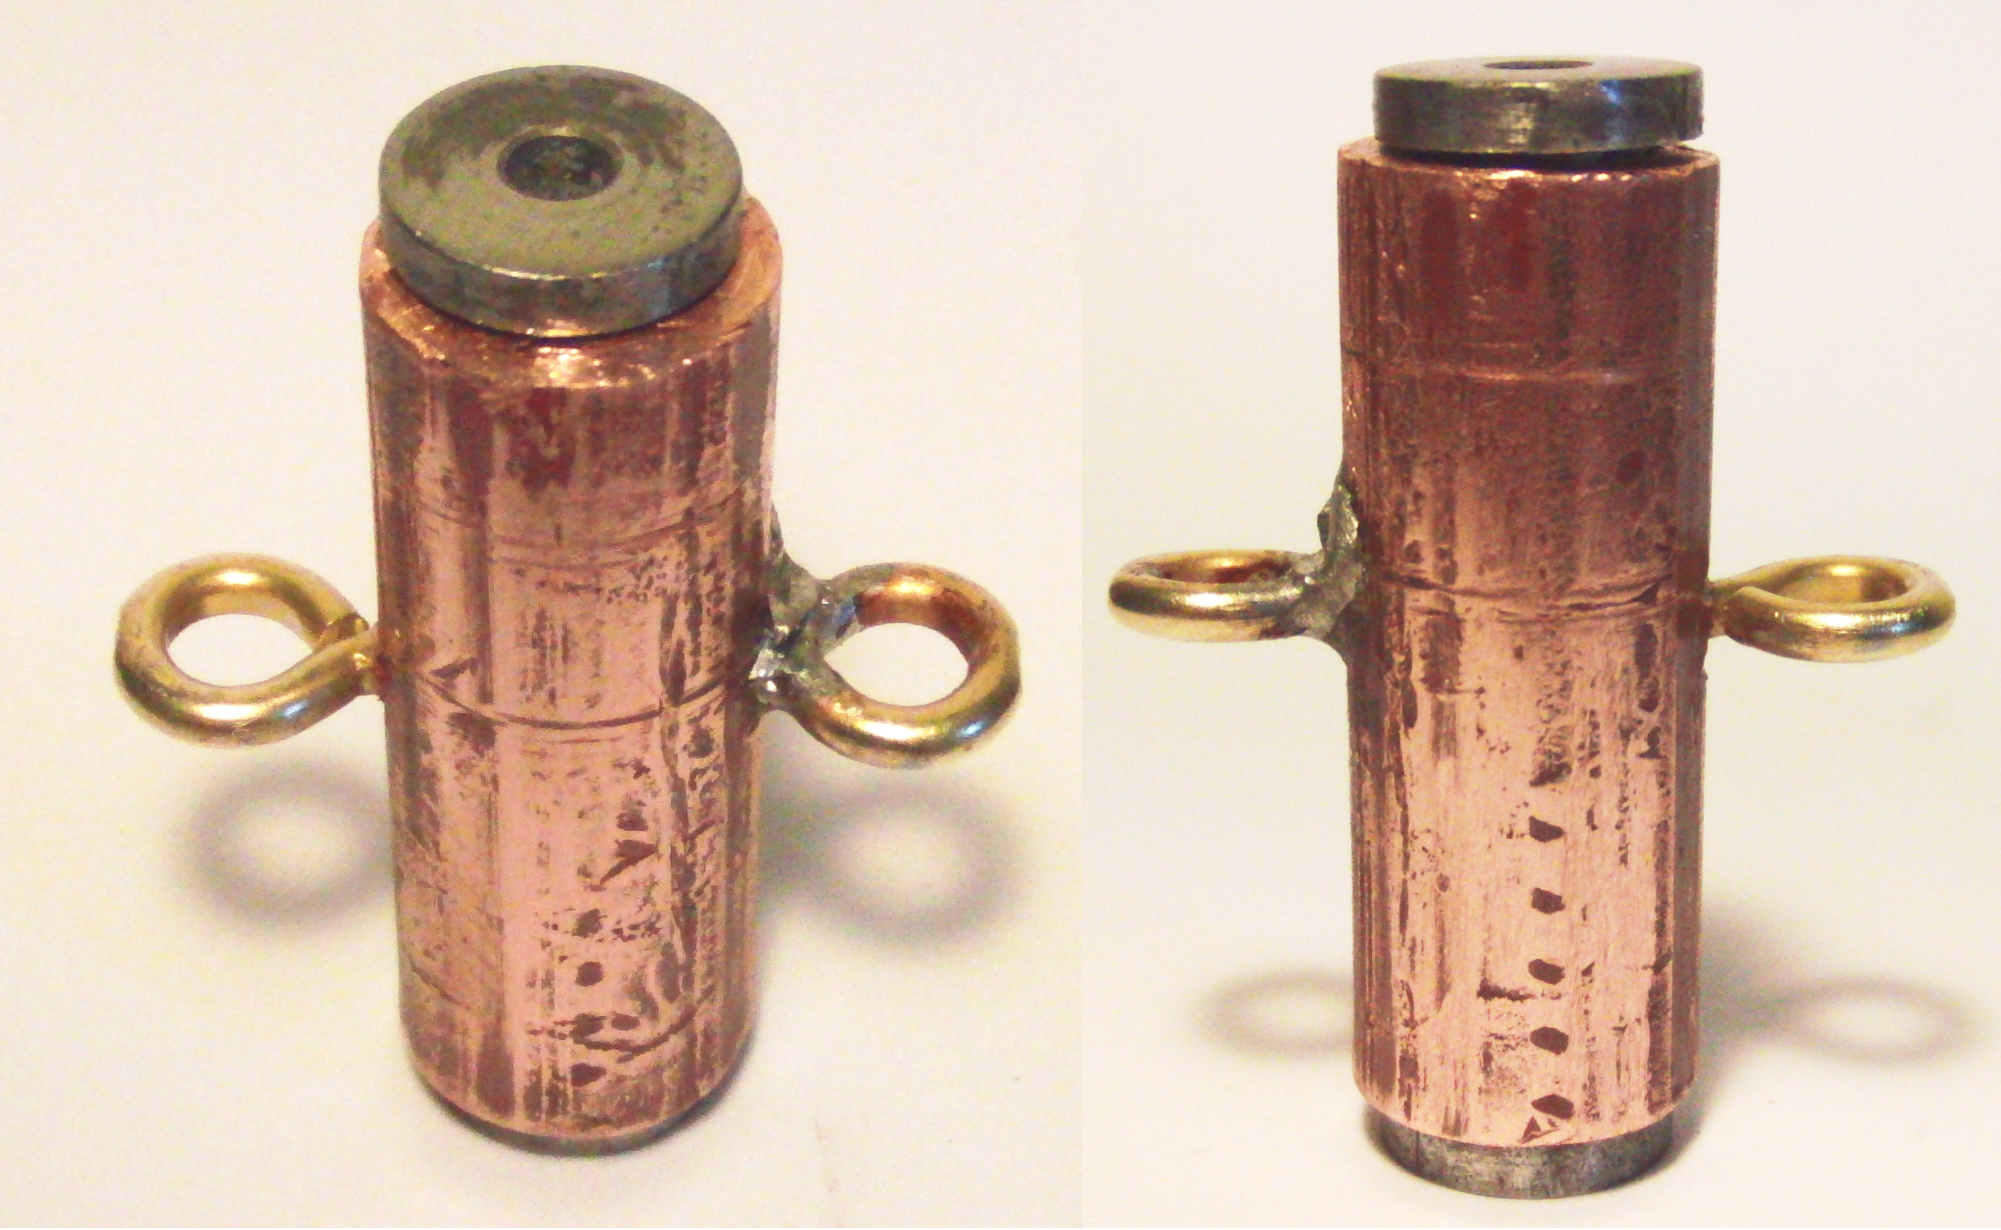
\includegraphics[width=0.8\textwidth]{./Immagini/sonda.png}
 % sonda.png: 2001x1230 pixel, 72dpi, 70.59x43.39 cm, bb=0 0 2001 1230
 \label{fig:sonda_verticale}
\end{figure}




\section*{Moto di un grave incatenato}

In questa esperienza vedremo come il moto di un grave incatenato si discosta da quello di un corpo in caduta libera. Tramite il sensore di posizione verticale misureremo lo spostamento della massa collegata alla catena, quindi dall'analisi delle posizioni dell'oggetto calcoleremo la velocità e l'accelerazione e analizzeremo come queste si discostano da quelle di una massa in caduta libera.
\begin{figure}[H]
 \centering
 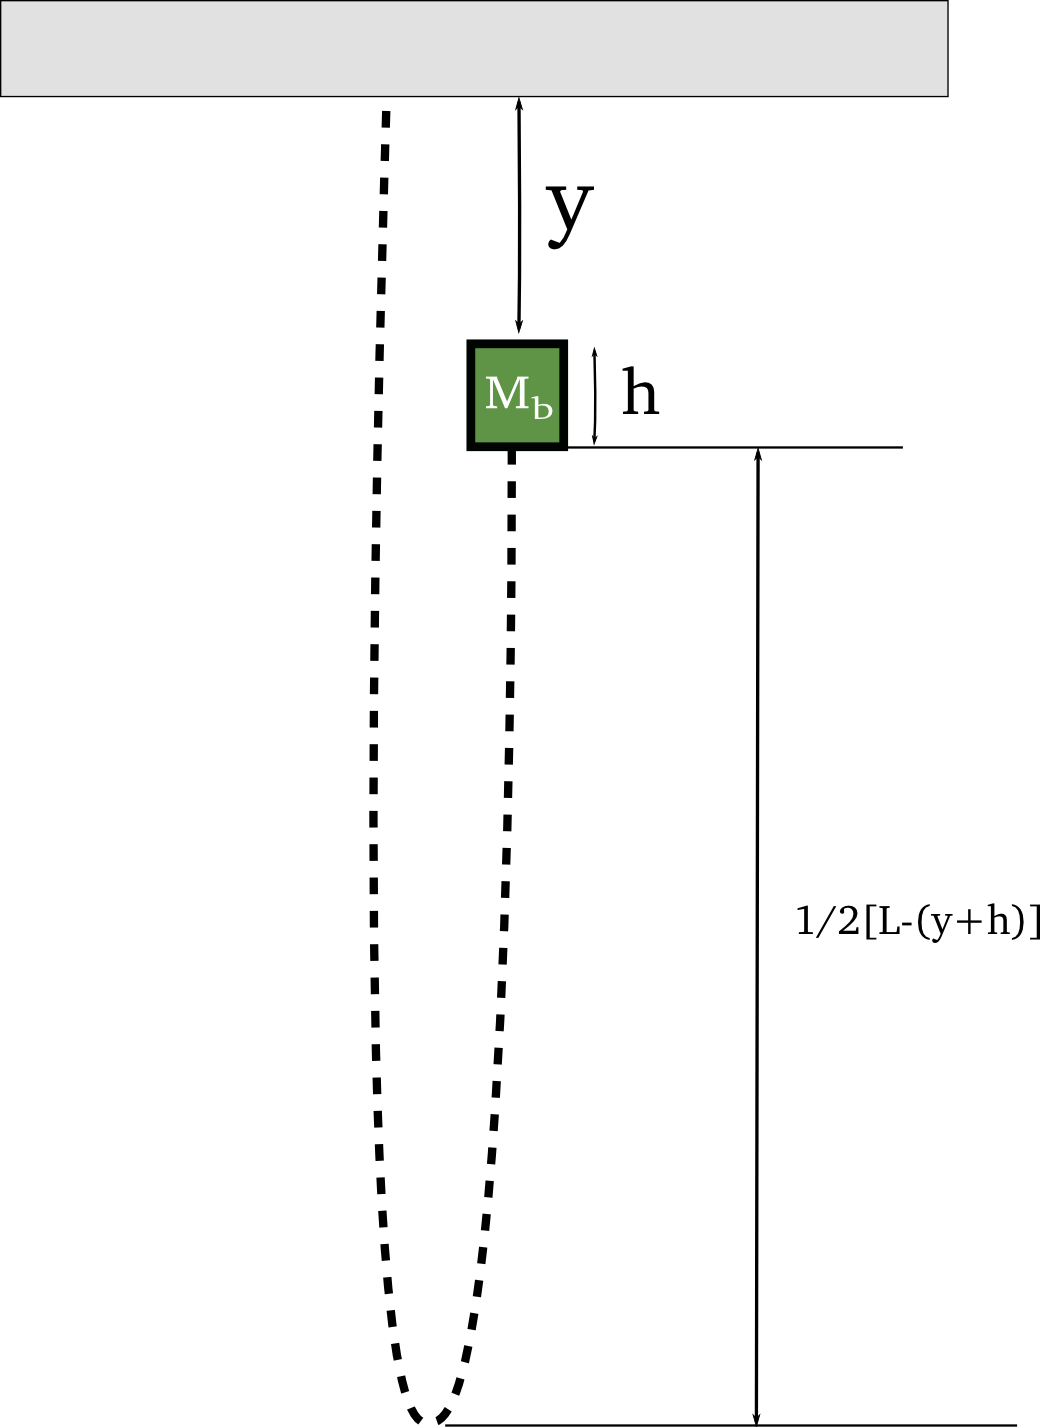
\includegraphics[width=0.6\textwidth]{./Immagini/bungiie.png}
 % bungiie.png: 1040x1427 pixel, 300dpi, 8.81x12.08 cm, bb=0 0 250 342
 \caption{Esperimento per la determinazione del moto di un grave incatenato}
 \label{fig:moto_incatenato}
\end{figure}

Possiamo meglio comprendere questo comportamento notando che per fermare gli anelli della catena in prossimità del punto di inversione deve essere esercitata una forza verso l'alto (sia dalla parte di catena fissata al soffitto che dalla parte di catena in caduta libera) per il terzo principio della dinamica l'elemento di catena in fase di rallentamento eserciterà una forza uguale ed opposta sulla parte sospesa e sulla parte in caduta. La massa della catena e del blocco in fase di caduta possono essere espresse come:
\begin{equation}
 M(t)=M_b+\frac{1}{2}(L-y(t))\lambda
\end{equation}

mentre la forza esercitata dall'elemento frenato sul sistema in caduta può essere espressa come:
\begin{equation}
 F_T=\frac{\lambda}{4}v^2(t)
\end{equation}
Utilizzando queste informazioni è possibile scrivere l'equazione del moto del sistema massa+catena,\footnote{L'equazione del moto risulta essere: 
\begin{equation}
 M(t)g=\frac 1 2 \dot{M}(t)v(t)+M(t)a(t)
\end{equation}
}
e ricavare l'accelerazione e la velocità del sistema ad una data quota, sfortunatamente non è possibile scrivere la dipendenza temporale di accelerazione e velocità in termini di funzioni elementari. In laboratorio cercheremo di ottenere sperimentalmente la dipendenza temporale di velocità ed accelerazione che confronteremo con quelle del moto di caduta libera.



\end{document}
